% Figure from MATH 591 notes, section 70. After the board (Lecture 25): relaunching the flow near the end (user's figure).
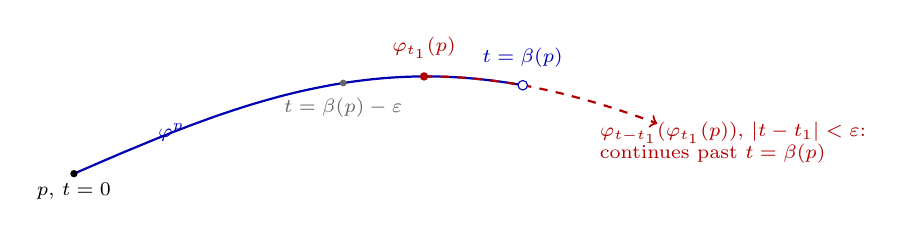
\begin{tikzpicture}[scale=0.95]
\draw[thick, blue!70!black] plot[smooth] coordinates {(-3.000,0.000) (-2.898,0.044) (-2.797,0.088) (-2.695,0.132) (-2.593,0.176) (-2.492,0.219) (-2.390,0.263) (-2.288,0.306) (-2.186,0.348) (-2.085,0.390) (-1.983,0.432) (-1.881,0.474) (-1.780,0.514) (-1.678,0.555) (-1.576,0.594) (-1.475,0.633) (-1.373,0.671) (-1.271,0.708) (-1.169,0.745) (-1.068,0.781) (-0.966,0.815) (-0.864,0.849) (-0.763,0.882) (-0.661,0.914) (-0.559,0.945) (-0.458,0.974) (-0.356,1.003) (-0.254,1.031) (-0.153,1.057) (-0.051,1.082) (0.051,1.106) (0.153,1.128) (0.254,1.149) (0.356,1.169) (0.458,1.188) (0.559,1.205) (0.661,1.221) (0.763,1.235) (0.864,1.248) (0.966,1.260) (1.068,1.270) (1.169,1.279) (1.271,1.286) (1.373,1.292) (1.475,1.296) (1.576,1.299) (1.678,1.300) (1.780,1.300) (1.881,1.298) (1.983,1.295) (2.085,1.290) (2.186,1.284) (2.288,1.276) (2.390,1.267) (2.492,1.256) (2.593,1.244) (2.695,1.231) (2.797,1.216) (2.898,1.200) (3.000,1.182)};
\draw[thick, red!70!black, dashed, ->] plot[smooth] coordinates {(1.680,1.300) (1.788,1.300) (1.895,1.298) (2.003,1.294) (2.110,1.289) (2.218,1.282) (2.326,1.273) (2.433,1.263) (2.541,1.251) (2.648,1.237) (2.756,1.222) (2.863,1.205) (2.971,1.187) (3.079,1.168) (3.186,1.146) (3.294,1.124) (3.401,1.099) (3.509,1.074) (3.617,1.047) (3.724,1.018) (3.832,0.989) (3.939,0.958) (4.047,0.926) (4.154,0.893) (4.262,0.858) (4.370,0.823) (4.477,0.786) (4.585,0.748) (4.692,0.710) (4.800,0.670)};
\fill (-3.000,0.000) circle (1.4pt) node[below, font=\scriptsize] {$p$, $t = 0$};
\draw[blue!70!black, fill=white] (3.000,1.182) circle (1.8pt) node[above=3pt, font=\scriptsize] {$t = \beta(p)$};
\fill[black!60] (0.600,1.212) circle (1.3pt) node[below=2pt, font=\scriptsize] {$t = \beta(p) - \varepsilon$};
\fill[red!70!black] (1.680,1.300) circle (1.6pt) node[above=3pt, font=\scriptsize] {$\varphi_{t_1}(p)$};
\node[blue!70!black, font=\scriptsize] at (-1.7,0.55) {$\varphi^p$};
\node[red!70!black, font=\scriptsize, anchor=north west, align=left] at (3.900,0.819) {$\varphi_{t - t_1}(\varphi_{t_1}(p))$, $|t - t_1| < \varepsilon$:\\ continues past $t = \beta(p)$};
\end{tikzpicture}
